% !TeX root = ..\..\rapport_13_1.tex
\section{Kravspecifikation}
\subsection{Indledning}
Denne del af rapporten dokumenterer de usecases og begreber som med udgangspunkt i projektoplægget, danner kravspecifikationerne for projektet. Use cases udvikles til Cucumber scenarier som igennem Behavior- og Test Driven Development bliver til den implementering som findes i anden rapport.
\subsection{Ordliste}
\begin{table}[H]
    \centering
    \setlength{\extrarowheight}{8pt}
    \begin{tabular}{>{\bfseries}l p{0.73\textwidth}}
        Medarbejder             & \textit{[Employee]} En medarbejder er en entitet ansat i Softwarehuset A/S, som har et unikt medarbejder ID (medarbejder initialer). En medarbejder kan påtage sig en projektleder rolle, oprette projekter, faste aktiviteter, projektaktiviteter og registrere arbejdstid på aktiviteter.                                    \\
        Projekt aktivitet       & \textit{[Project activity]} En delopgave af et projekt. Aktiviteter har en start- og slutuge, og kan få fastsat en budgetteret tid. Alle medarbejdere kan udføre arbejde på alle projektaktiviteter.                                                                                                                           \\
        Fast aktivitet          & \textit{[Regular activity]} Aktivitet der ikke kan pålægges et projekt. F.eks. ferie, sygdom, kurser. Disse har en start- og slutuge.                                                                                                                                                                                          \\
        Projekt                 & \textit{[Project]} Udviklingsarbejde udført for en kunde. Et projekt administreres af en projektleder og er inddelt i aktiviteter. Hvert projekt har et projektnummer.                                                                                                                                                         \\
        Kunde                   & \textit{[Customer]} En ekstern entitet som bestiller og er modtager af projekter.                                                                                                                                                                                                                                              \\
        Projektleder            & \textit{[Project leader]} En medarbejder der har ret til at oprette og tildele aktiviteter for et givent projekt samt generere projektrapporter.                                                                                                                                                                               \\
        Medarbejder initialer   & \textit{[Employee initials]} Unik identifikation for hver enkelt medarbejder, bestående af fire bogstaver. To første fra fornavn efterfulgt af to første fra efternavn. F.eks. ``rawi''. Hvis initialer allerede er taget, vælges bogstav et og tre i efternavn, derefter et og fire, osv.                                     \\
        Projektnummer           & \textit{[Project number]} Identifikation for hvert enkelt projekt. Har formen årstal efterfulgt af et trecifret løbenummer. F.eks. ``23001''                                                                                                                                                                                   \\
        Budgetteret tid         & \textit{[Time budget]} En aktivitets estimerede antal hele timer.                                                                                                                                                                                                                                                              \\
        Arbejdstidsregistrering & \textit{[Work time registration]} Mængde tid i inkrementer af halve timer, brugt på en aktivitet. Kan registreres af den medarbejder som har brugt arbejdstid på en given aktivitet.                                                                                                                                           \\
        Start- og sluttid       & \textit{[Start- and end week]} En periode med opløsning på uge-niveau til aktiviteter. Begge tider angives som år og uge, ved formatet ``ÅÅUU''. F.eks. 2304 for uge 4 i 2023. En starttid afgrænser starten af en given uge, en sluttid afgrænser ved slutningen af en given uge. Start- og sluttid kan derfor godt være ens. \\
        Projektrapport          & \textit{[Project report]} Et udskrift der viser info om et projekt, (Leder, kunde, projekt ID), samt aktiviteter, deres arbejdstidsregistreringer og samlede fremgang.
    \end{tabular}
\end{table}\newpage
\subsection{Use case diagrammer}
Dette afsnit starter med \cref{fig:AlleActorsPaaEnGang} som viser hvilke aktører der kan udfører hvilke cases. Herefter kommer en oversigt (\cref{tbl:oversigt}) over de detaljerede use cases med henvisning til Cucumber features (\cpagerefrange{lst:usecaseRegisterEmployee}{lst:usecaseGenerateProjectReport2}) og sekvensdiagrammer (\Cpagerefrange{fig:sequenceRegisterEmployee}{fig:sequenceGenerateProjectReport}).
% \begin{figure}[H]
%     \centering
%     \caption{Use case diagram for programmet hvori de tre aktører inkluderet er Gæst, Medarbejder og Projektleder.}\label{fig:AlleActorsPaaEnGang}
%     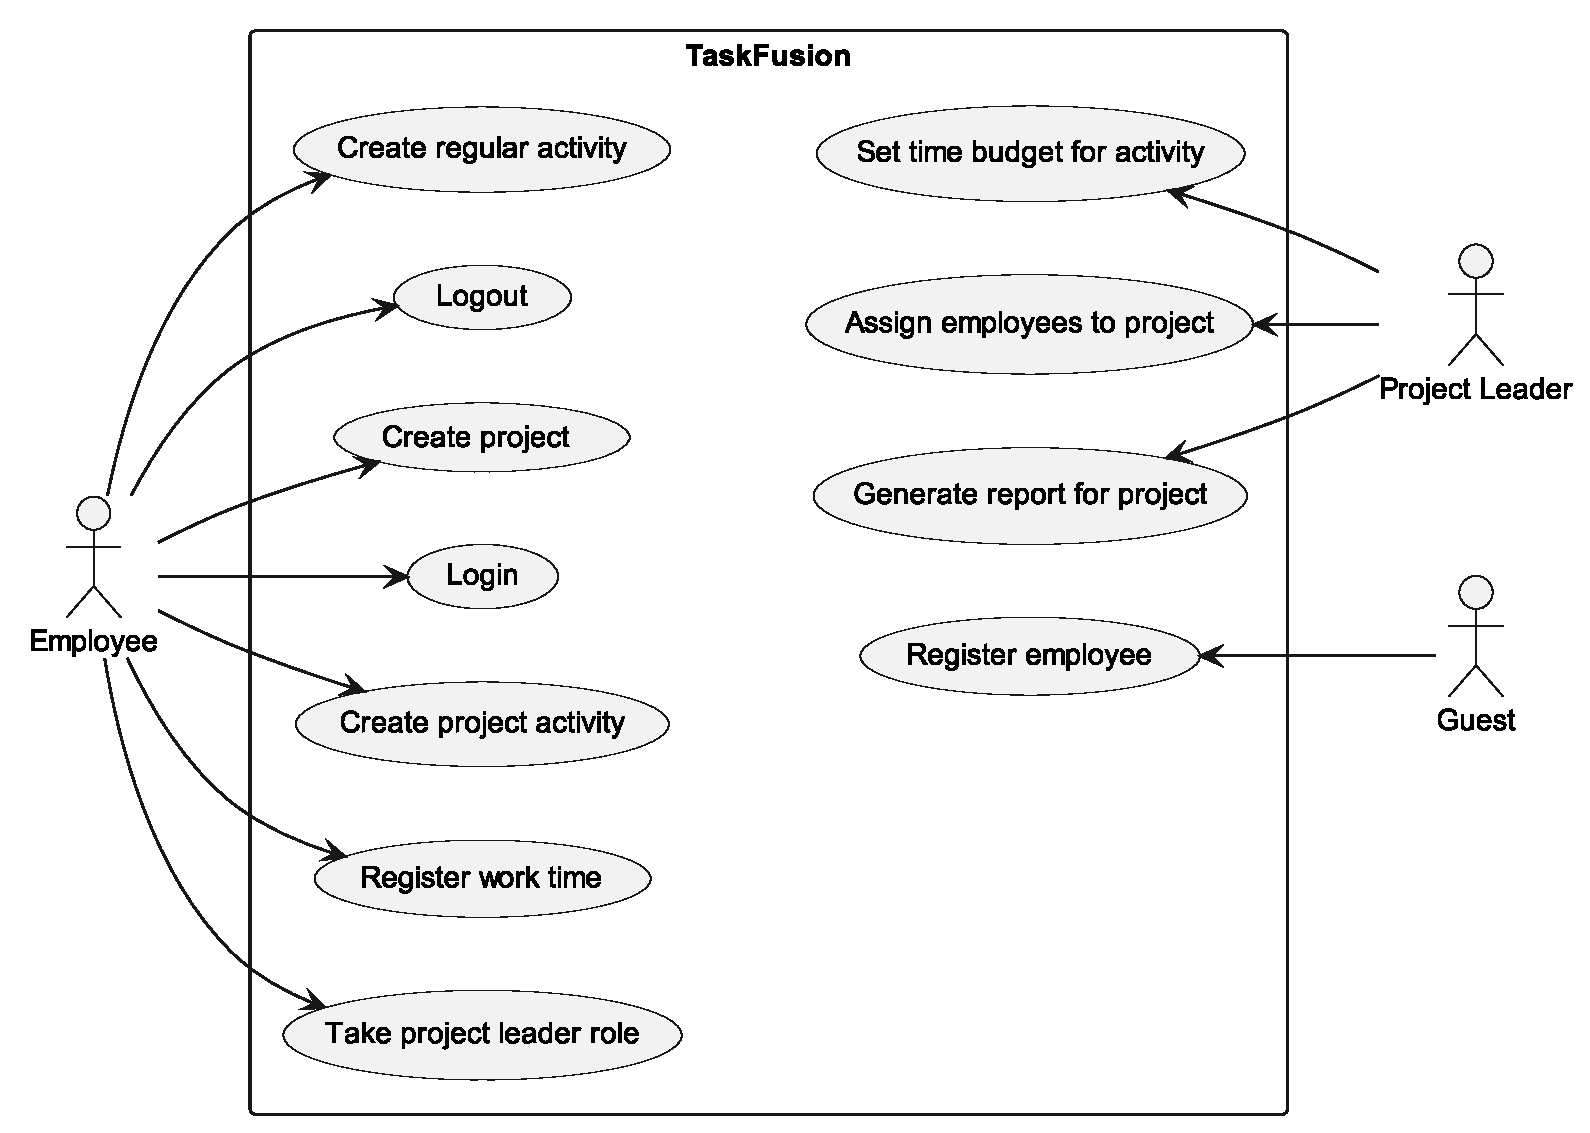
\includegraphics[width=.85\textwidth]{RequirementsAndDesign/Diagrams/usecases.eps}
% \end{figure}
\begin{figure}[H]
    \centering
    \caption{Use case diagrammer for programmet hvori de tre aktører inkluderet er Gæst, Medarbejder og Projektleder.}\label{fig:AlleActorsPaaEnGang}
    \begin{subfigure}[c]{.5\textwidth}
        \centering
        \caption{Use cases for medarbejder}
        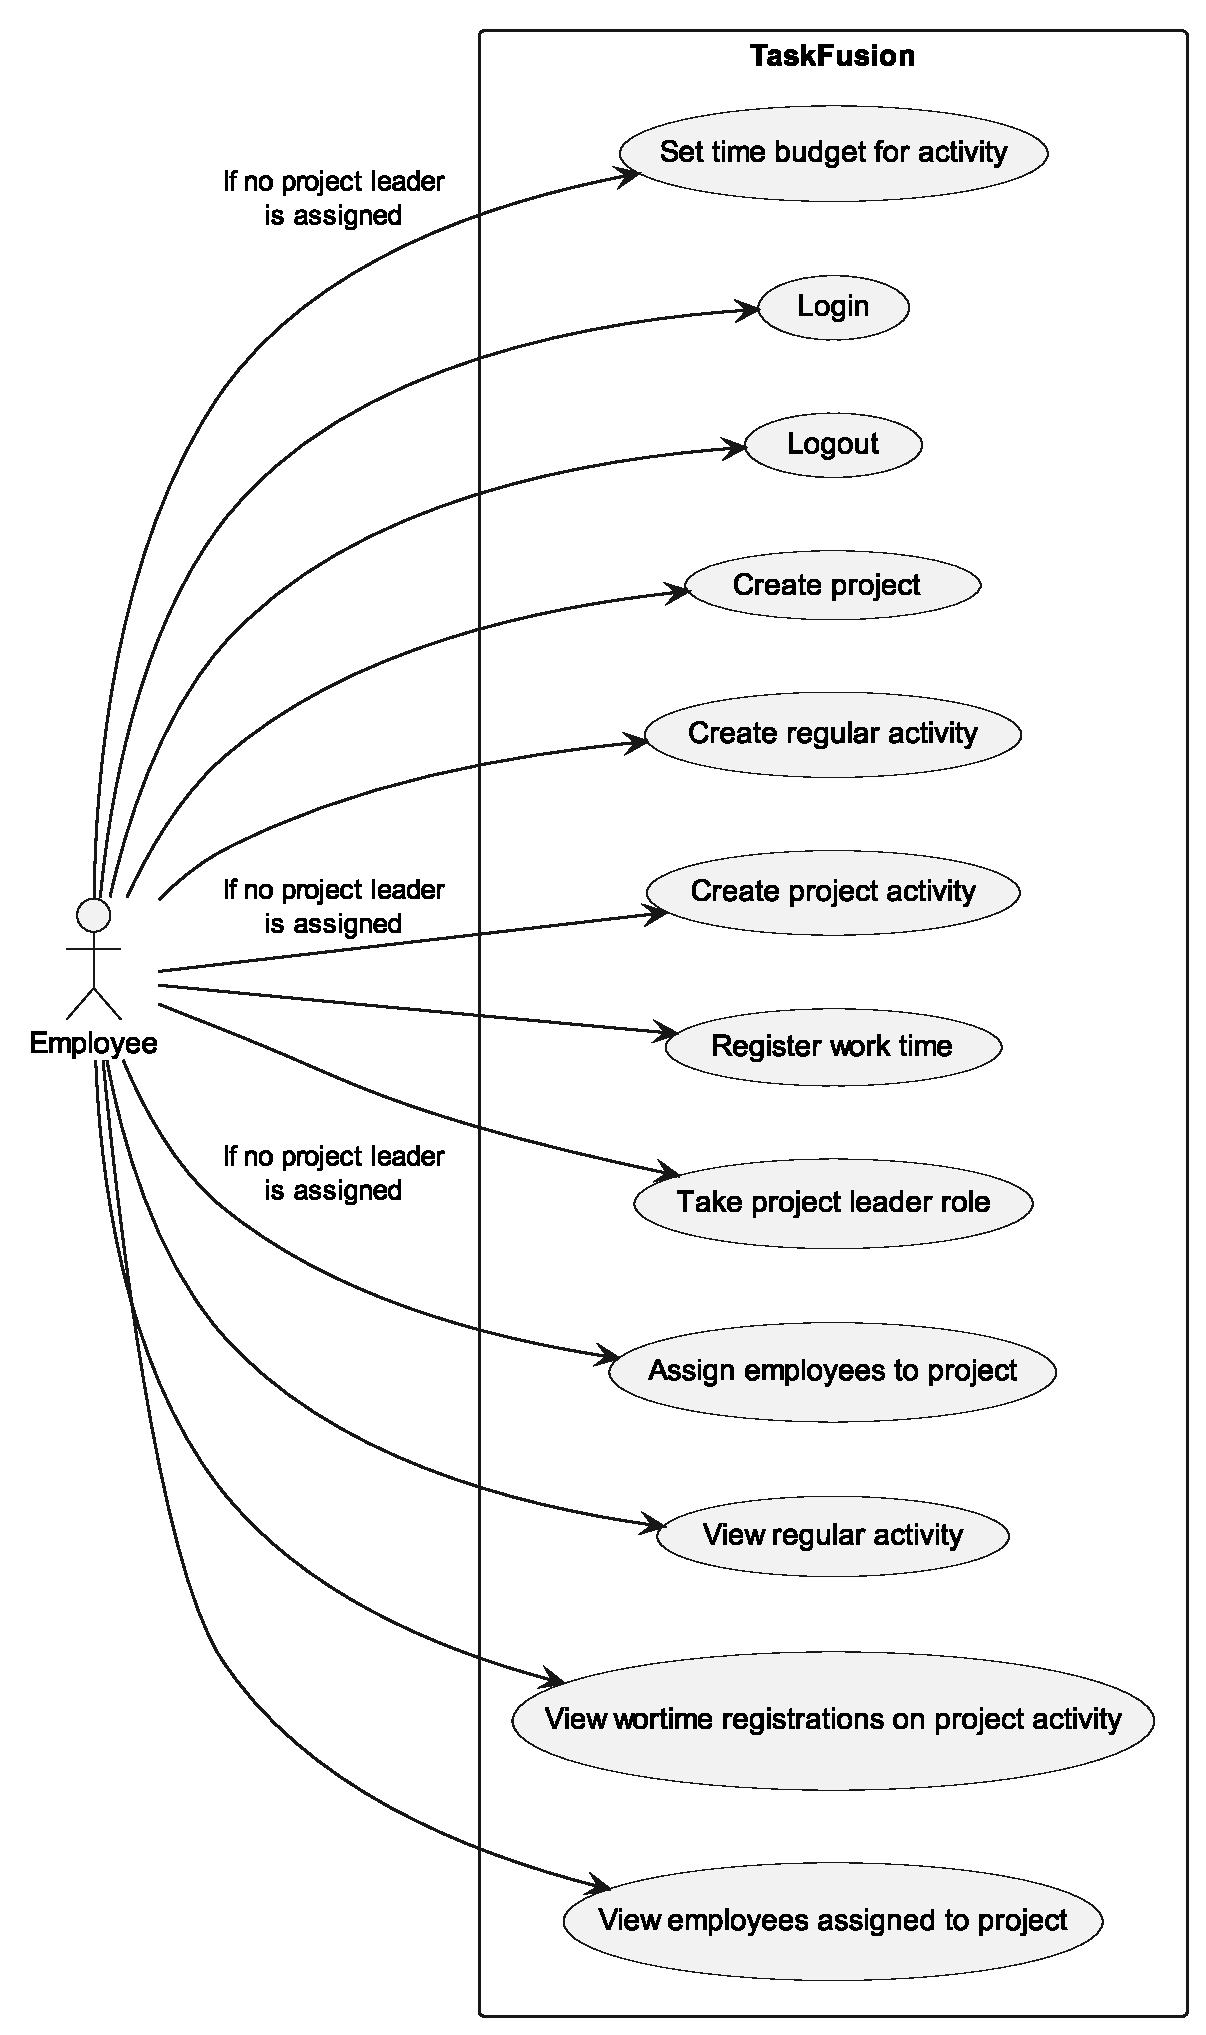
\includegraphics[width=\textwidth]{RequirementsAndDesign/Diagrams/usecasesEmployee.eps}\label{fig:ucEmployee}
    \end{subfigure}
    \qquad
    \begin{subfigure}[c]{.4\textwidth}
        \centering
        \caption{Use cases for gæst}
        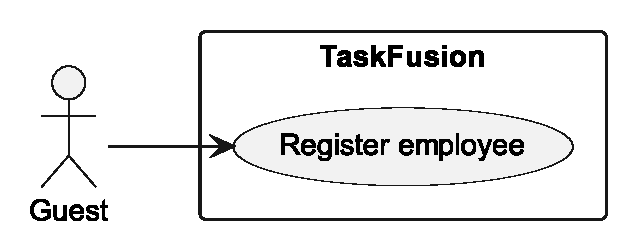
\includegraphics[width=.8\textwidth]{RequirementsAndDesign/Diagrams/usecasesGuest.eps}\label{fig:ucGuest}

        \vspace{10ex}

        \caption{Use cases for projektleder}
        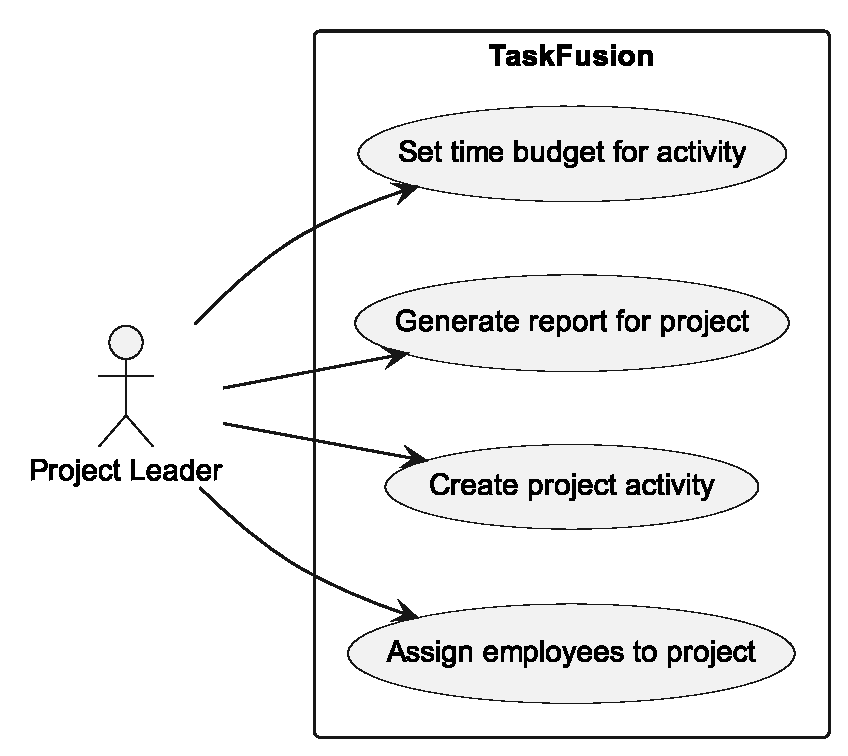
\includegraphics[width=\textwidth]{RequirementsAndDesign/Diagrams/usecasesProjectLeader.eps}\label{fig:ucProjectLeader}
    \end{subfigure}
\end{figure}

Som beskrevet i \cref{fig:AlleActorsPaaEnGang} har vi tre roller: Medarbejder (\cref{fig:ucEmployee}), gæst (\cref{fig:ucGuest}) og projektleder (\cref{fig:ucProjectLeader}). Gæsten er en indgang til et system uden data og kan kun oprette medarbejdere i systemet. Medarbejdere har rettigheder til stort set alle funktioner i programmet, indtil en projektleder udpeges. Herefter er det kun projektlederen på et projekt, der kan tilføje medarbejdere til projektet, oprette projektaktiviteter, angive tidsbudgetter og generere rapporter.
\begin{table}[H]
    \centering
    \caption{Use cases for programmet}\label{tbl:oversigt}
    \begin{tabular}{lll}
        \toprule
        Detaljeret use case                           & Cucumber feature                                                                                                                & Sekvensdiagram                           \\
        \midrule
        Opret medarbejder                             & \cref{lst:usecaseRegisterEmployee}                                                                                              & \cref{fig:sequenceRegisterEmployee}      \\
        Login                                         & \cref{lst:usecaseLogin}                                                                                                         & \cref{fig:sequenceLogin}                 \\
        Logout                                        & \cref{lst:usecaseLogout}                                                                                                        & \cref{fig:sequenceLogout}                \\
        Opret projekt                                 & \cref{lst:usecaseCreateProject1,,lst:usecaseCreateProject2}                                                                     & \cref{fig:sequenceCreateProject}         \\
        Påtag projektlederrolle                       & \cref{lst:usecaseTakePLRole}                                                                                                    & \cref{fig:sequenceTakePLRole}            \\
        Tildel medarbejder til projekt                & \cref{lst:usecaseAssignEmployee}                                                                                                & \cref{fig:sequenceAssignEmployee}        \\
        Se medarbejdere tilknyttet et projekt         & \cref{lst:usecaseViewAssignedEmployee}                                                                                          & \cref{fig:ViewAssignedEmployee}          \\
        Opret projektaktivitet                        & \cref{lst:usecaseCreateProjectActivityPL,,lst:usecaseCreateProjectActivityEmployee1,,lst:usecaseCreateProjectActivityEmployee2} & \cref{fig:sequenceCreateProjectActivity} \\
        Anfør tidsbudget på projektaktivitet          & \cref{lst:usecaseSetTimeBudget}                                                                                                 & \cref{fig:sequenceSetTimeBudget}         \\
        Opret fast aktivitet                          & \cref{lst:usecaseCreateRegularActivity1,,lst:usecaseCreateRegularActivity2}                                                     & \cref{fig:sequenceCreateRegularActivity} \\
        Se fast aktivitet                             & \cref{lst:usecaseViewRegularActivity}                                                                                           & \cref{fig:sequenceViewRegularActivity}   \\
        Registrer arbejdstid                          & \cref{lst:usecaseRegisterWorktime1,,lst:usecaseRegisterWorktime2}                                                               & \cref{fig:sequenceRegisterWorktime}      \\
        Se registreret arbejdstid på projektaktivitet & \cref{lst:RemainingWork,,lst:usecaseViewWorktime1,,lst:usecaseViewWorktime2}                                                    & \cref{fig:sequenceViewWorktime}          \\
        Generér projektrapport                        & \cref{lst:usecaseGenerateProjectReport1,,lst:usecaseGenerateProjectReport2}                                                     & \cref{fig:sequenceGenerateProjectReport} \\
        \bottomrule
    \end{tabular}
\end{table}
\subsection{Detaljerede use cases}
\begin{listing}[H]
    \centering
    \caption{Cucumber feature: Opret medarbejder}\label{lst:usecaseRegisterEmployee}
    \inputminted[breaklines]{cucumber}{TaskFusion/features/employees/register_employee.feature}
\end{listing}
\begin{listing}[H]
    \centering
    \caption{Cucmber feature: Login}\label{lst:usecaseLogin}
    \inputminted[breaklines]{cucumber}{TaskFusion/features/employees/login.feature}
\end{listing}
\begin{listing}[H]
    \centering
    \caption{Cucmber feature: Logout}\label{lst:usecaseLogout}
    \inputminted[breaklines]{cucumber}{TaskFusion/features/employees/logout.feature}
\end{listing}
\begin{listing}[H]
    \centering
    \caption{Cucmber feature: Opret projekt (fortsætter på \cref{lst:usecaseCreateProject2})}\label{lst:usecaseCreateProject1}
    \inputminted[breaklines, lastline=36]{cucumber}{TaskFusion/features/projects/create_project.feature}
\end{listing}
\begin{listing}[H]
    \centering
    \caption{Cucmber feature: Opret projekt (fortsat fra \cref{lst:usecaseCreateProject1})}\label{lst:usecaseCreateProject2}
    \inputminted[breaklines, firstline=37]{cucumber}{TaskFusion/features/projects/create_project.feature}
\end{listing}
\begin{listing}[H]
    \centering
    \caption{Cucumber feature: Påtag projektlederrolle}\label{lst:usecaseTakePLRole}
    \inputminted[breaklines]{cucumber}{TaskFusion/features/projects/assign_project_leader_to_project.feature}
\end{listing}
\begin{listing}[H]
    \centering
    \caption{Cucmber feature: Tildel medarbejder til projekt}\label{lst:usecaseAssignEmployee}
    \inputminted[breaklines]{cucumber}{TaskFusion/features/projects/assign_employee_to_project.feature}
\end{listing}
\begin{listing}[H]
    \centering
    \caption{Cucumber feature: Se medarbejdere tilknyttet et projekt}\label{lst:usecaseViewAssignedEmployee}
    \inputminted[breaklines]{cucumber}{TaskFusion/features/projects/get_list_participating_employees.feature}
\end{listing}
\begin{listing}[H]
    \centering
    \caption{Cucmber feature: Opret projektaktivitet som projektleder}\label{lst:usecaseCreateProjectActivityPL}
    \inputminted[breaklines]{cucumber}{TaskFusion/features/activities/create_project_activity_with_leader.feature}
\end{listing}
\begin{listing}[H]
    \centering
    \caption{Cucmber feature: Opret projektaktivitet som medarbejder (fortsætter på \cref{lst:usecaseCreateProjectActivityEmployee2})}\label{lst:usecaseCreateProjectActivityEmployee1}
    \inputminted[breaklines, lastline=46]{cucumber}{TaskFusion/features/activities/create_project_activity_without_leader.feature}
\end{listing}
\begin{listing}[H]
    \centering
    \caption{Cucmber feature: Opret projektaktivitet som medarbejder (fortsat fra \cref{lst:usecaseCreateProjectActivityEmployee1})}\label{lst:usecaseCreateProjectActivityEmployee2}
    \inputminted[breaklines, firstline=47]{cucumber}{TaskFusion/features/activities/create_project_activity_without_leader.feature}
\end{listing}
\begin{listing}[H]
    \centering
    \caption{Cucmber feature: Anfør tidsbudget på projektaktivitet}\label{lst:usecaseSetTimeBudget}
    \inputminted[breaklines]{cucumber}{TaskFusion/features/activities/activity_work_time_budget.feature}
\end{listing}
\begin{listing}[H]
    \centering
    \caption{Cucmber feature: Opret fast aktivitet (fortsætter på \cref{lst:usecaseCreateRegularActivity2})}\label{lst:usecaseCreateRegularActivity1}
    \inputminted[breaklines, lastline=16]{cucumber}{TaskFusion/features/regular_activities/create_regular_activity.feature}
\end{listing}
\begin{listing}[H]
    \centering
    \caption{Cucmber feature: Opret fast aktivitet (fortsat fra \cref{lst:usecaseCreateRegularActivity1})}\label{lst:usecaseCreateRegularActivity2}
    \inputminted[breaklines, firstline=17]{cucumber}{TaskFusion/features/regular_activities/create_regular_activity.feature}
\end{listing}
\begin{listing}[H]
    \centering
    \caption{Cucumber feature: Se fast aktivitet}\label{lst:usecaseViewRegularActivity}
    \inputminted[breaklines]{cucumber}{TaskFusion/features/regular_activities/view_regular_activity.feature}
\end{listing}
\begin{listing}[H]
    \centering
    \caption{Cucmber feature: Registrer arbejdstid (fortsætter på \cref{lst:usecaseRegisterWorktime2})}\label{lst:usecaseRegisterWorktime1}
    \inputminted[breaklines, lastline=33]{cucumber}{TaskFusion/features/activities/register_activity_work_time.feature}
\end{listing}
\begin{listing}[H]
    \centering
    \caption{Cucmber feature: Registrer arbejdstid (fortsat fra \cref{lst:usecaseRegisterWorktime1})}\label{lst:usecaseRegisterWorktime2}
    \inputminted[breaklines, firstline=34]{cucumber}{TaskFusion/features/activities/register_activity_work_time.feature}
\end{listing}
\begin{listing}[H]
    \centering
    \caption{Cucumber feature: Se resterende arbejdstid}\label{lst:RemainingWork}
    \inputminted[breaklines]{cucumber}{TaskFusion/features/activities/activity_remaining_work.feature}
\end{listing}
\begin{listing}[H]
    \centering
    \caption{Cucumber feature: Se registreret arbejdstid på projektaktivitet (fortsætter på \cref{lst:usecaseViewWorktime2})}\label{lst:usecaseViewWorktime1}
    \inputminted[breaklines, lastline=44]{cucumber}{TaskFusion/features/activities/overview_work_time.feature}
\end{listing}
\begin{listing}[H]
    \centering
    \caption{Cucumber feature: Se registreret arbejdstid på projektaktivitet (fortsat fra \cref{lst:usecaseViewWorktime1})}\label{lst:usecaseViewWorktime2}
    \inputminted[breaklines, firstline=45]{cucumber}{TaskFusion/features/activities/overview_work_time.feature}
\end{listing}
\begin{listing}[H]
    \centering
    \caption{Cucmber feature: Generer projektrapport (fortsætter på \cref{lst:usecaseGenerateProjectReport2})}\label{lst:usecaseGenerateProjectReport1}
    \inputminted[breaklines, lastline=32]{cucumber}{TaskFusion/features/reports/create_report.feature}
\end{listing}
\begin{listing}[H]
    \centering
    \caption{Cucmber feature: Generer projektrapport (fortsat fra \cref{lst:usecaseGenerateProjectReport1})}\label{lst:usecaseGenerateProjectReport2}
    \inputminted[breaklines, firstline=33]{cucumber}{TaskFusion/features/reports/create_report.feature}
\end{listing}\newpage
\section{Diskussion: Kravspecifikation}
\subsection{Oplægsmæssige overvejelser og afgrænsninger}
\subsubsection{En admin rolle}
Oplægget nævner som udgangspunkt ikke et krav om en administrator rolle, men derimod at det er et internt system og at der ikke er behov for et sikkerhedslag. Ofte er det oplagt at have en admin entitet, og i dette projekt kunne det som eksempel give mening til oprettelse af medarbejdere. Men i forbindelse med en kortlægning af projektet samt afgrænsning af funktioner, ser vi større værdi for kunden i at fokusere på de ønskede funktioner i stedet for at \textit{gætte} på at de vil have en admin. Desuden kan en sådan rolle laves senere, hvis nødvendigt. At en gæst kan oprette en medarbejder er dermed et eksempel på brugen af K.I.S.S. \footnote{(\textbf{K}eep \textbf{I}t \textbf{S}hort and \textbf{S}imple, some also refer to it as \textbf{K}eep \textbf{I}t \textbf{S}imple, \textbf{S}tupid)} ved at anskue denne funktionalitet som en mock admin-klasse, der eksisterer udelukkende i forbindelse med udviklingen af arbejdstidsregistrering og projekthåndtering, de centrale ønsker.
\subsubsection{UI og fokus på business logik}
Oplægget kræver en brugerflade, men giver frit lejde til hvorvidt denne skal være en GUI eller CLI. Vi ønsker at levere noget brugbart til kunden hurtigt, og have K.I.S.S. i fokus for vores beslutninger og afgrænsning. Fra tidlige leverancer kan vi bruge kundens feedback til at videreudvikle på softwareløsningen iterativt, og bedre kunne prioritere udvikling af funktioner løbende. Derfor har vi i første ikke noget grafisk bruger interface, men derimod et program der køres i et CLI. På et senere stadie, i samtale med kunden, kan en grafisk brugerflade implementeres.
\subsubsection{Medarbejdere med samme navn}
For at tilgodese at medarbejdere kan hedde det samme vil medarbejder-objekter blive gemt ud fra deres initialer \textbf{som derfor skal være unikke}.
\subsection{Tekniske overvejelser}
\subsubsection{Abstractions og compositions}
Disse to begreber bliver kun brugt i abstrakt forstand, da man i Java ikke har direkte kontrol over objekter. De kan konstrueres, men eksistere selv når objekter der peger på dem slettes. Java har en garbage collector der jævnligt analysere pointers i programmet og fjerner objekter der ikke bliver peget på.
\subsubsection{Persistence}
For at gøre det muligt at gemme data i objekter og være sikker på at kun disse objekter konstrueres vil singletons blive brugt som indgang til gemt information. Dette kan optimeres ved at gemme data på filer, men dette har vi valgt ikke at fokusere på, for at få tid til funktionalitet.
\subsubsection{Adskillelse af UI fra business logik}
UI'en er som nævnt tekstbaseret. Hele UI-laget er separeret fra business logikken igennem \textit{Facades}, og vil kunne se objekter som \textit{ModelView}-klasser der ikke kan ændre på underliggende data men blot læse disse.\newpage